\partlabel{PART V --- USER MANUAL (TWO PAGES)}
\chapter{Installation and Configuration}
\section{Requirements and startup}
Use Docker Engine/Compose, CPU/RAM/disk for local models and PostgreSQL. Images use Node 24/Python 3.12; native npm requires Node \texttt{\^{}22.13.0 || >=24}. No minimum RAM is specified. From the root, copy \texttt{.env.example} \emph{only if no .env exists}, fill secrets and protect permissions. Preserve existing initialized database passwords.
\begin{lstlisting}[language=bash]
cp .env.example .env                 # new checkout only
chmod 600 .env
docker network create meta-harness-mcp # once, if absent
docker compose -f docker-compose.yml -f docker-compose.mcp.yml up -d --build --wait
(cd rag-server && docker compose --env-file ../.env -f docker-compose.yml -f docker-compose.meta-harness.yml up -d --build --wait)
# New installation only: create the dedicated external volume.
docker volume create manufacturing-demo_manufacturing-data
(cd zsk-service && docker compose --env-file ../.env -f docker-compose.yml -f docker-compose.meta-harness.yml up -d --build --wait)
\end{lstlisting}
Required root secrets are \texttt{DB\_PASSWORD}, \texttt{OPENAI\_API\_KEY} (or enter in UI), \texttt{RAG\_DB\_PASSWORD}, \texttt{RAG\_API\_KEY}, \texttt{MANUFACTURING\_DB\_PASSWORD}, \texttt{ZSK\_API\_KEY} and \texttt{ZSK\_ADMIN\_API\_KEY}. Use distinct ZSK read/admin keys of at least 16 characters and a RAG API key of at least 32 characters. Use \texttt{LLM\_MODEL}/\texttt{LLM\_THINKING} through UI. Keep the MCP overlay on later core startup commands. If replacing the old demo, stop it \emph{without deleting volumes} before ZSK; never run two DB containers on its volume.
\section{Configure real UI connections}
Open \url{http://localhost:8080}; core health is \url{http://localhost:8000/api/health}, RAG REST is port 8090 and ZSK port 8100. Expand \textbf{LLM}: Save API key, select an available Model/Thinking, Save settings. Unsupported combinations fail visibly.

Under \textbf{MCP > Connections/Add MCP Server}, use \texttt{http://manufacturing-ml:8000/mcp} for containerized core and bearer reference \texttt{ZSK\_API\_KEY}. Save, Test Connection/Discover Tools, allow the five reads and enable agent use; Save tool permissions. Under \textbf{RAG > Connection}, use MCP \texttt{http://rag-api:8090/mcp} and REST \texttt{http://rag-api:8090}; save/test and allow four read tools. Existing profiles retain credentials; new tokens are write-only entries. Operator-approved exact origins must be in root .env.
\begin{center}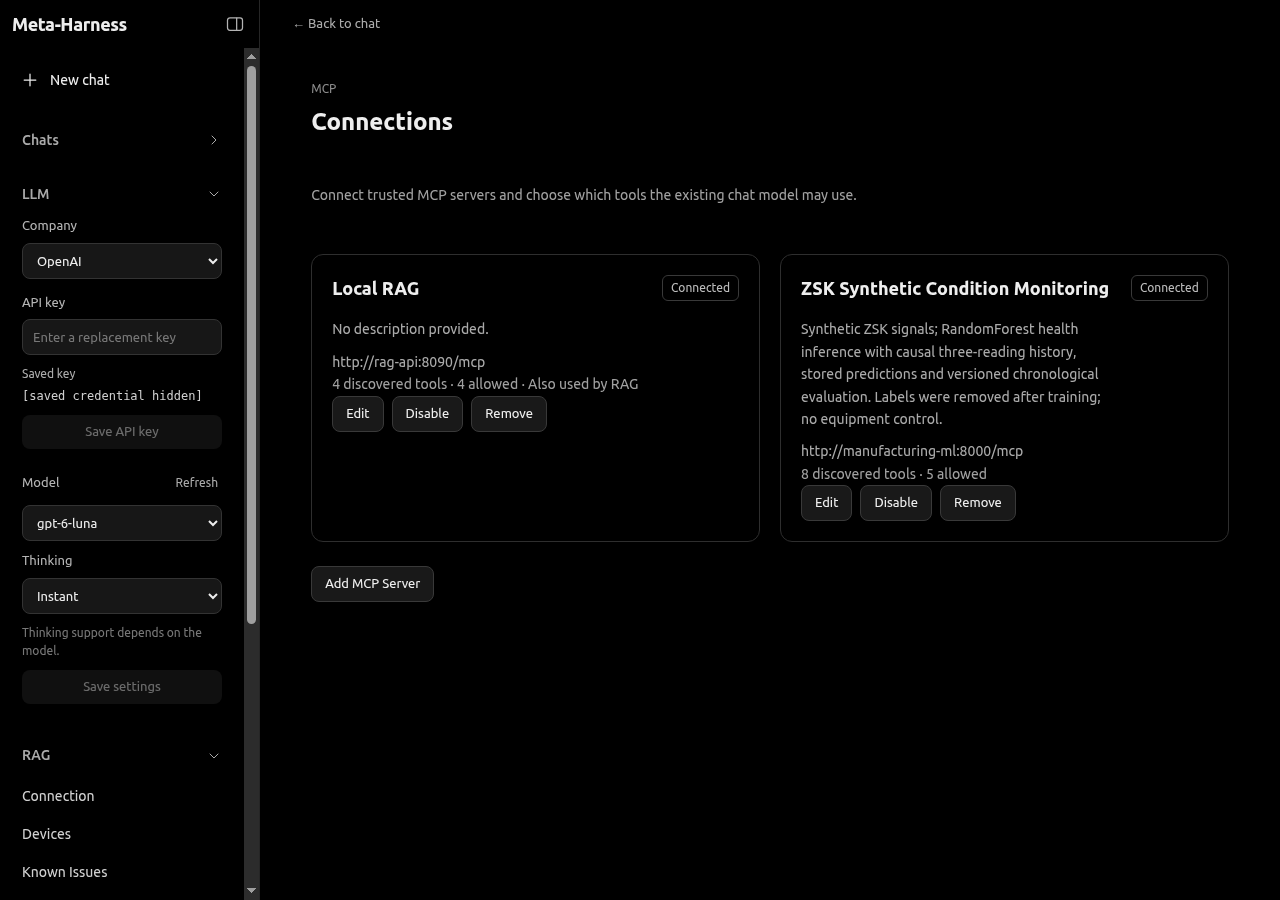
\includegraphics[width=.94\linewidth,trim=310bp 345bp 40bp 250bp,clip]{screenshots/connections.png}\captionof{figure}{Detail from a genuine repository capture of connected RAG/ZSK profiles (9 October 2026). Saved credential metadata was hidden in the supplied publication capture.}\end{center}
